% Options for packages loaded elsewhere
\PassOptionsToPackage{unicode}{hyperref}
\PassOptionsToPackage{hyphens}{url}
%
\documentclass[
  ignorenonframetext,
]{beamer}
\usepackage{pgfpages}
\setbeamertemplate{caption}[numbered]
\setbeamertemplate{caption label separator}{: }
\setbeamercolor{caption name}{fg=normal text.fg}
\beamertemplatenavigationsymbolsempty
% Prevent slide breaks in the middle of a paragraph
\widowpenalties 1 10000
\raggedbottom
\setbeamertemplate{part page}{
  \centering
  \begin{beamercolorbox}[sep=16pt,center]{part title}
    \usebeamerfont{part title}\insertpart\par
  \end{beamercolorbox}
}
\setbeamertemplate{section page}{
  \centering
  \begin{beamercolorbox}[sep=12pt,center]{part title}
    \usebeamerfont{section title}\insertsection\par
  \end{beamercolorbox}
}
\setbeamertemplate{subsection page}{
  \centering
  \begin{beamercolorbox}[sep=8pt,center]{part title}
    \usebeamerfont{subsection title}\insertsubsection\par
  \end{beamercolorbox}
}
\AtBeginPart{
  \frame{\partpage}
}
\AtBeginSection{
  \ifbibliography
  \else
    \frame{\sectionpage}
  \fi
}
\AtBeginSubsection{
  \frame{\subsectionpage}
}

\usepackage{amsmath,amssymb}
\usepackage{lmodern}
\usepackage{iftex}
\ifPDFTeX
  \usepackage[T1]{fontenc}
  \usepackage[utf8]{inputenc}
  \usepackage{textcomp} % provide euro and other symbols
\else % if luatex or xetex
  \usepackage{unicode-math}
  \defaultfontfeatures{Scale=MatchLowercase}
  \defaultfontfeatures[\rmfamily]{Ligatures=TeX,Scale=1}
\fi
% Use upquote if available, for straight quotes in verbatim environments
\IfFileExists{upquote.sty}{\usepackage{upquote}}{}
\IfFileExists{microtype.sty}{% use microtype if available
  \usepackage[]{microtype}
  \UseMicrotypeSet[protrusion]{basicmath} % disable protrusion for tt fonts
}{}
\makeatletter
\@ifundefined{KOMAClassName}{% if non-KOMA class
  \IfFileExists{parskip.sty}{%
    \usepackage{parskip}
  }{% else
    \setlength{\parindent}{0pt}
    \setlength{\parskip}{6pt plus 2pt minus 1pt}}
}{% if KOMA class
  \KOMAoptions{parskip=half}}
\makeatother
\usepackage{xcolor}
\newif\ifbibliography
\setlength{\emergencystretch}{3em} % prevent overfull lines
\setcounter{secnumdepth}{-\maxdimen} % remove section numbering

\usepackage{color}
\usepackage{fancyvrb}
\newcommand{\VerbBar}{|}
\newcommand{\VERB}{\Verb[commandchars=\\\{\}]}
\DefineVerbatimEnvironment{Highlighting}{Verbatim}{commandchars=\\\{\}}
% Add ',fontsize=\small' for more characters per line
\usepackage{framed}
\definecolor{shadecolor}{RGB}{241,243,245}
\newenvironment{Shaded}{\begin{snugshade}}{\end{snugshade}}
\newcommand{\AlertTok}[1]{\textcolor[rgb]{0.68,0.00,0.00}{#1}}
\newcommand{\AnnotationTok}[1]{\textcolor[rgb]{0.37,0.37,0.37}{#1}}
\newcommand{\AttributeTok}[1]{\textcolor[rgb]{0.40,0.45,0.13}{#1}}
\newcommand{\BaseNTok}[1]{\textcolor[rgb]{0.68,0.00,0.00}{#1}}
\newcommand{\BuiltInTok}[1]{\textcolor[rgb]{0.00,0.23,0.31}{#1}}
\newcommand{\CharTok}[1]{\textcolor[rgb]{0.13,0.47,0.30}{#1}}
\newcommand{\CommentTok}[1]{\textcolor[rgb]{0.37,0.37,0.37}{#1}}
\newcommand{\CommentVarTok}[1]{\textcolor[rgb]{0.37,0.37,0.37}{\textit{#1}}}
\newcommand{\ConstantTok}[1]{\textcolor[rgb]{0.56,0.35,0.01}{#1}}
\newcommand{\ControlFlowTok}[1]{\textcolor[rgb]{0.00,0.23,0.31}{#1}}
\newcommand{\DataTypeTok}[1]{\textcolor[rgb]{0.68,0.00,0.00}{#1}}
\newcommand{\DecValTok}[1]{\textcolor[rgb]{0.68,0.00,0.00}{#1}}
\newcommand{\DocumentationTok}[1]{\textcolor[rgb]{0.37,0.37,0.37}{\textit{#1}}}
\newcommand{\ErrorTok}[1]{\textcolor[rgb]{0.68,0.00,0.00}{#1}}
\newcommand{\ExtensionTok}[1]{\textcolor[rgb]{0.00,0.23,0.31}{#1}}
\newcommand{\FloatTok}[1]{\textcolor[rgb]{0.68,0.00,0.00}{#1}}
\newcommand{\FunctionTok}[1]{\textcolor[rgb]{0.28,0.35,0.67}{#1}}
\newcommand{\ImportTok}[1]{\textcolor[rgb]{0.00,0.46,0.62}{#1}}
\newcommand{\InformationTok}[1]{\textcolor[rgb]{0.37,0.37,0.37}{#1}}
\newcommand{\KeywordTok}[1]{\textcolor[rgb]{0.00,0.23,0.31}{#1}}
\newcommand{\NormalTok}[1]{\textcolor[rgb]{0.00,0.23,0.31}{#1}}
\newcommand{\OperatorTok}[1]{\textcolor[rgb]{0.37,0.37,0.37}{#1}}
\newcommand{\OtherTok}[1]{\textcolor[rgb]{0.00,0.23,0.31}{#1}}
\newcommand{\PreprocessorTok}[1]{\textcolor[rgb]{0.68,0.00,0.00}{#1}}
\newcommand{\RegionMarkerTok}[1]{\textcolor[rgb]{0.00,0.23,0.31}{#1}}
\newcommand{\SpecialCharTok}[1]{\textcolor[rgb]{0.37,0.37,0.37}{#1}}
\newcommand{\SpecialStringTok}[1]{\textcolor[rgb]{0.13,0.47,0.30}{#1}}
\newcommand{\StringTok}[1]{\textcolor[rgb]{0.13,0.47,0.30}{#1}}
\newcommand{\VariableTok}[1]{\textcolor[rgb]{0.07,0.07,0.07}{#1}}
\newcommand{\VerbatimStringTok}[1]{\textcolor[rgb]{0.13,0.47,0.30}{#1}}
\newcommand{\WarningTok}[1]{\textcolor[rgb]{0.37,0.37,0.37}{\textit{#1}}}

\providecommand{\tightlist}{%
  \setlength{\itemsep}{0pt}\setlength{\parskip}{0pt}}\usepackage{longtable,booktabs,array}
\usepackage{calc} % for calculating minipage widths
\usepackage{caption}
% Make caption package work with longtable
\makeatletter
\def\fnum@table{\tablename~\thetable}
\makeatother
\usepackage{graphicx}
\makeatletter
\def\maxwidth{\ifdim\Gin@nat@width>\linewidth\linewidth\else\Gin@nat@width\fi}
\def\maxheight{\ifdim\Gin@nat@height>\textheight\textheight\else\Gin@nat@height\fi}
\makeatother
% Scale images if necessary, so that they will not overflow the page
% margins by default, and it is still possible to overwrite the defaults
% using explicit options in \includegraphics[width, height, ...]{}
\setkeys{Gin}{width=\maxwidth,height=\maxheight,keepaspectratio}
% Set default figure placement to htbp
\makeatletter
\def\fps@figure{htbp}
\makeatother

\makeatletter
\makeatother
\makeatletter
\makeatother
\makeatletter
\@ifpackageloaded{caption}{}{\usepackage{caption}}
\AtBeginDocument{%
\ifdefined\contentsname
  \renewcommand*\contentsname{Table of contents}
\else
  \newcommand\contentsname{Table of contents}
\fi
\ifdefined\listfigurename
  \renewcommand*\listfigurename{List of Figures}
\else
  \newcommand\listfigurename{List of Figures}
\fi
\ifdefined\listtablename
  \renewcommand*\listtablename{List of Tables}
\else
  \newcommand\listtablename{List of Tables}
\fi
\ifdefined\figurename
  \renewcommand*\figurename{Figure}
\else
  \newcommand\figurename{Figure}
\fi
\ifdefined\tablename
  \renewcommand*\tablename{Table}
\else
  \newcommand\tablename{Table}
\fi
}
\@ifpackageloaded{float}{}{\usepackage{float}}
\floatstyle{ruled}
\@ifundefined{c@chapter}{\newfloat{codelisting}{h}{lop}}{\newfloat{codelisting}{h}{lop}[chapter]}
\floatname{codelisting}{Listing}
\newcommand*\listoflistings{\listof{codelisting}{List of Listings}}
\makeatother
\makeatletter
\@ifpackageloaded{caption}{}{\usepackage{caption}}
\@ifpackageloaded{subcaption}{}{\usepackage{subcaption}}
\makeatother
\makeatletter
\@ifpackageloaded{tcolorbox}{}{\usepackage[many]{tcolorbox}}
\makeatother
\makeatletter
\@ifundefined{shadecolor}{\definecolor{shadecolor}{rgb}{.97, .97, .97}}
\makeatother
\makeatletter
\makeatother
\ifLuaTeX
  \usepackage{selnolig}  % disable illegal ligatures
\fi
\IfFileExists{bookmark.sty}{\usepackage{bookmark}}{\usepackage{hyperref}}
\IfFileExists{xurl.sty}{\usepackage{xurl}}{} % add URL line breaks if available
\urlstyle{same} % disable monospaced font for URLs
\hypersetup{
  pdftitle={Simulating Environmental Drivers for Hake Recruitment Deviation Predictions},
  pdfauthor={Rachael Ren, UW; Dr.~Kiva Oken, NWFSC},
  hidelinks,
  pdfcreator={LaTeX via pandoc}}

\title{Simulating Environmental Drivers for Hake Recruitment Deviation
Predictions}
\author{Rachael Ren, UW; Dr.~Kiva Oken, NWFSC}
\date{}

\begin{document}
\frame{\titlepage}
\ifdefined\Shaded\renewenvironment{Shaded}{\begin{tcolorbox}[sharp corners, boxrule=0pt, enhanced, breakable, borderline west={3pt}{0pt}{shadecolor}, frame hidden, interior hidden]}{\end{tcolorbox}}\fi

\begin{frame}
\begin{block}{About Me}
\protect\hypertarget{about-me}{}
\begin{itemize}
\tightlist
\item
  Rising senior at the University of Washington majoring in Statistics,
  minoring in Environmental Studies
\end{itemize}

\pause

\begin{itemize}
\tightlist
\item
  Applying to Statistics PhD programs this Winter
\end{itemize}

\pause

\begin{itemize}
\tightlist
\item
  Leaning towards continuing this project during the school year (open
  to long-term suggestions)
\end{itemize}
\end{block}
\end{frame}

\begin{frame}{Background/Motivation}
\protect\hypertarget{backgroundmotivation}{}
\begin{block}{Recruitment Deviations}
\protect\hypertarget{recruitment-deviations}{}
\begin{figure}

{\centering \includegraphics[width=3.42708in,height=\textheight]{beverton-holt.PNG}

}

\caption{Kapur 2021}

\end{figure}

A \textbf{recruitment deviation} (rec dev) is a scaling factor
indicating how far off our observed data is from the theoretical curve

Hake recruitment is especially variable from year to year
\end{block}

\begin{block}{Environmental Drivers}
\protect\hypertarget{environmental-drivers}{}
We want to incorporate environmental drivers into hake recruitment
deviation predictions

``Our results suggest that the environment more strongly influences
recruitment than spawning biomass over the observed stock sizes for many
stocks.'' (Szuwalski)
\end{block}
\end{frame}

\begin{frame}{Research Question}
\protect\hypertarget{research-question}{}
\textbf{How correlated must an environmental driver be with past
recruitment deviations to improve future recruitment deviation
predictions?}

\pause

Hypothesis: As environmental drivers become increasingly correlated with
recruitment deviations, predictions will become increasingly accurate.
\end{frame}

\begin{frame}{Methods}
\protect\hypertarget{methods}{}
\end{frame}

\begin{frame}
Three types of stock synthesis models:

\begin{enumerate}
\item
  \textbf{Base model with all years (1946 to 2019)}
\item
  Base retrospective model
\item
  Environmentally-linked retrospective model
\end{enumerate}

\begin{figure}

{\centering 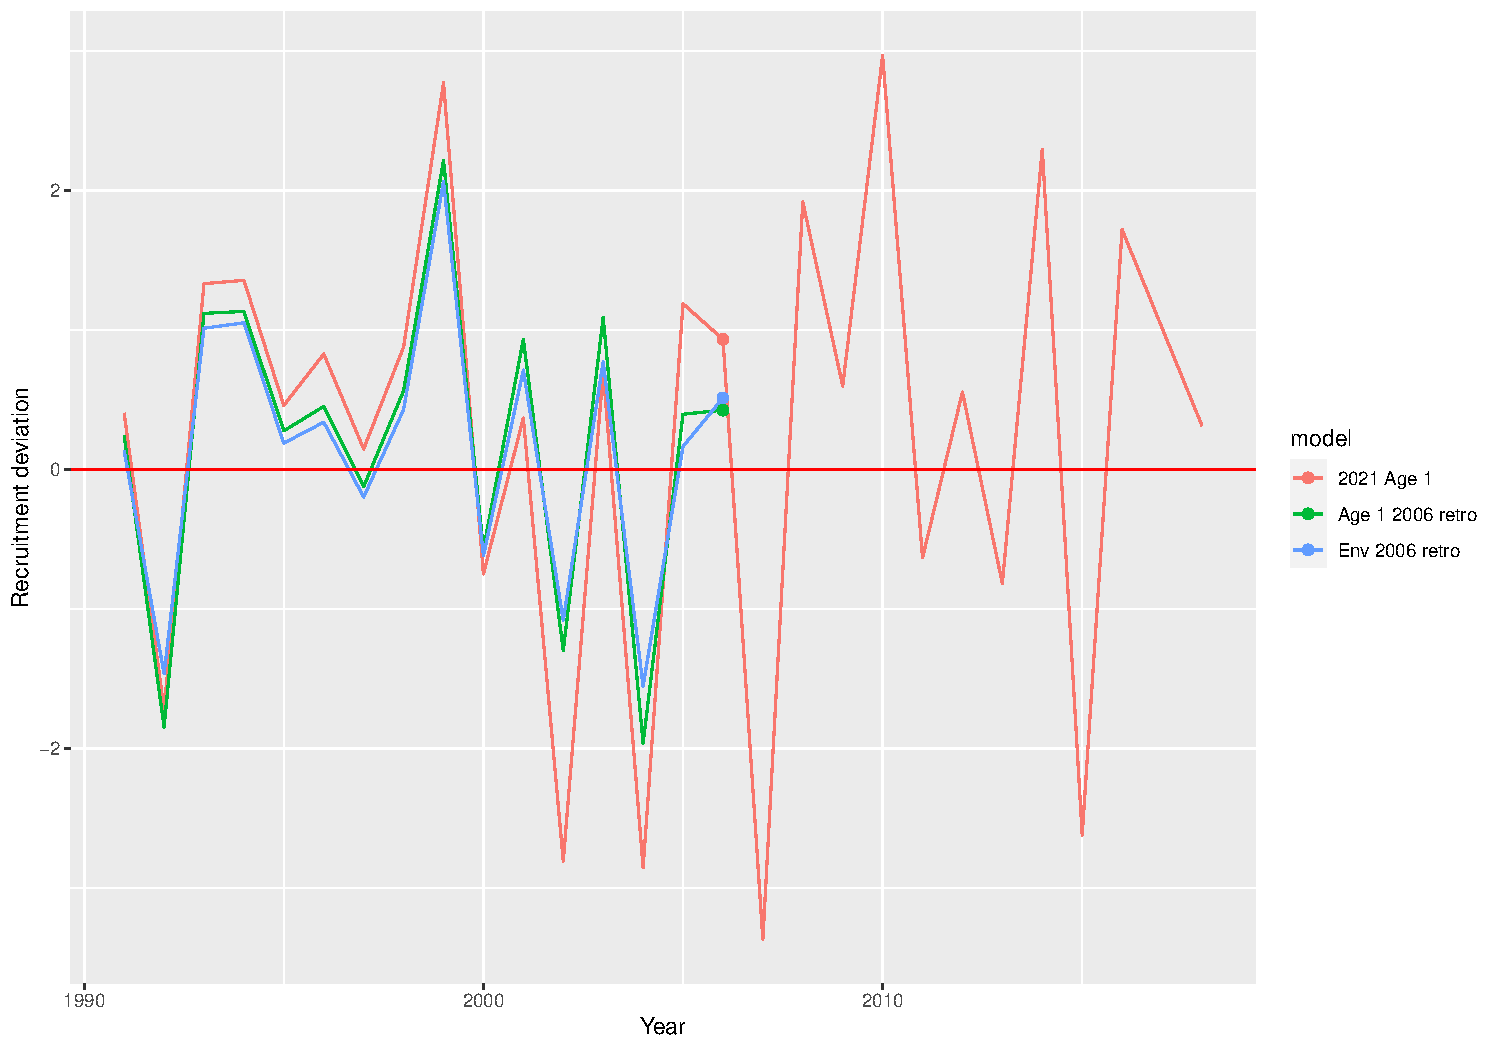
\includegraphics{presentation_files/figure-beamer/unnamed-chunk-1-1.pdf}

}

\end{figure}
\end{frame}

\begin{frame}
Assessment of accuracy: absolute difference in the terminal year

Which model is closer (has smaller absolute difference) to the ``true''
recruitment deviation in the terminal year?

\begin{figure}

{\centering 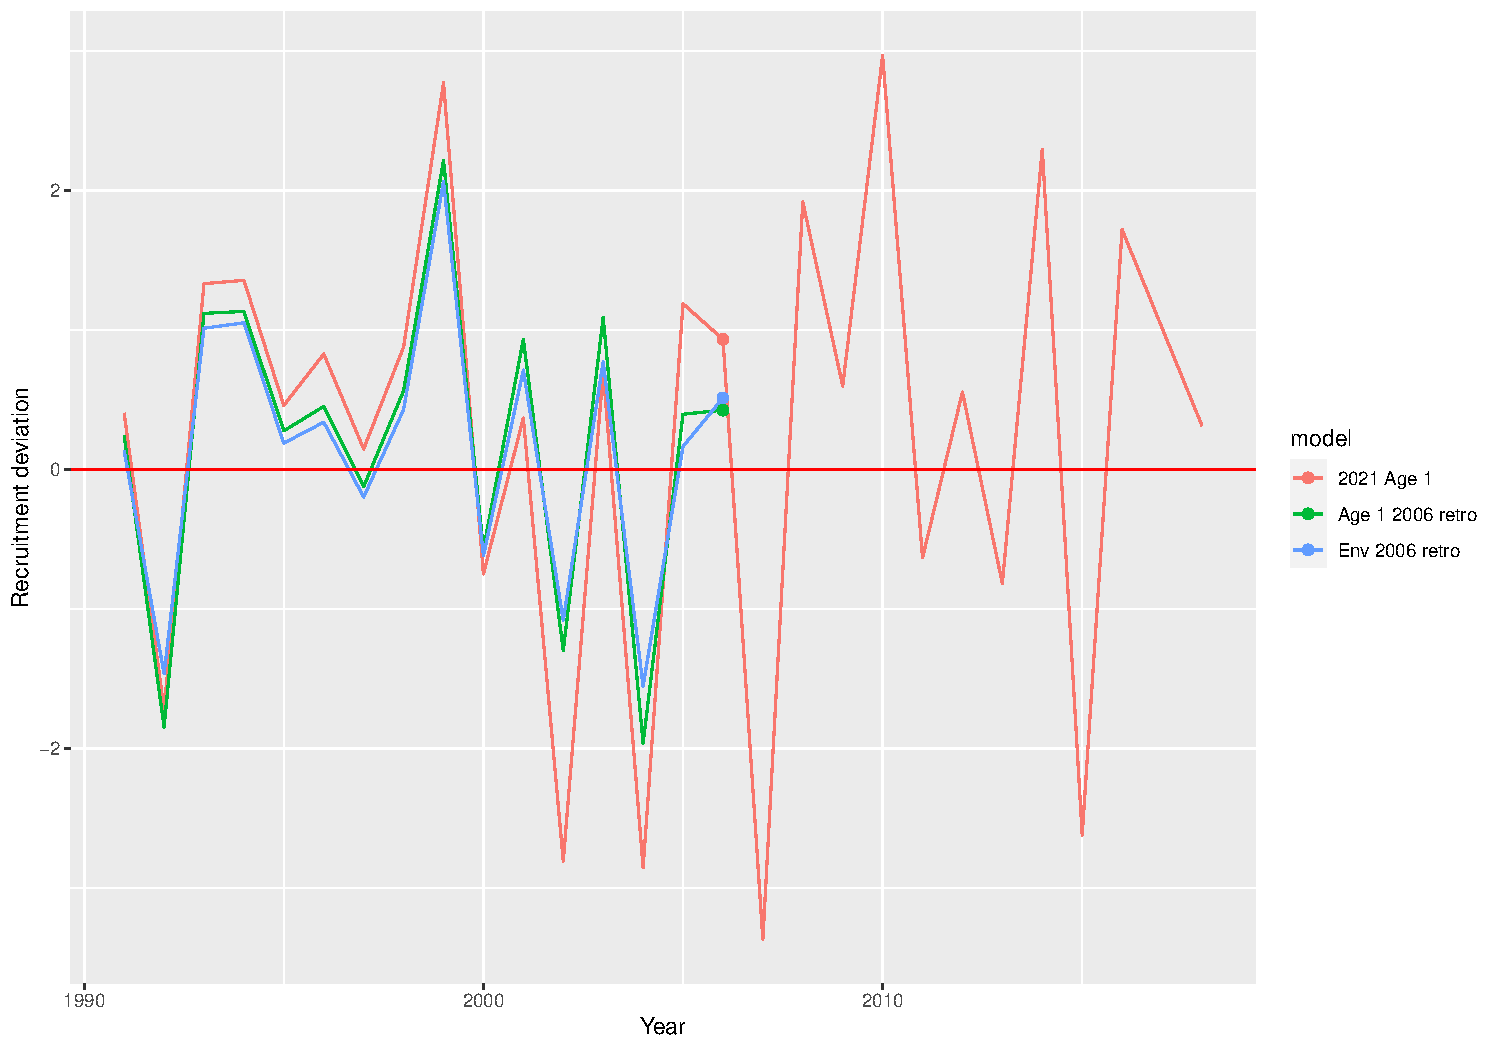
\includegraphics{presentation_files/figure-beamer/unnamed-chunk-2-1.pdf}

}

\end{figure}
\end{frame}

\begin{frame}
\begin{enumerate}
\tightlist
\item
  Simulate 50 fake environmental driver time series for each correlation
  level (0.25, 0.5, 0.75, 0.9)
\end{enumerate}

\pause

\begin{enumerate}
\setcounter{enumi}{1}
\tightlist
\item
  Run SS in MLE mode for:
\end{enumerate}

\begin{itemize}
\item
  Base model with all years (1)
\item
  Base model with 15 years peeled back (1)
\item
  Environmentally-linked models with 15 years peeled back (50 time
  series x 4 levels = 200 total)
\end{itemize}

\pause

\begin{enumerate}
\setcounter{enumi}{2}
\tightlist
\item
  Compare environmental errors with base error
\end{enumerate}
\end{frame}

\begin{frame}{Results}
\protect\hypertarget{results}{}
\end{frame}

\begin{frame}
\begin{figure}

{\centering \includegraphics[width=4.73958in,height=\textheight]{SE1.PNG}

}

\end{figure}
\end{frame}

\begin{frame}
Inputting exact recruitment deviations for the environmental driver:

\begin{figure}

{\centering 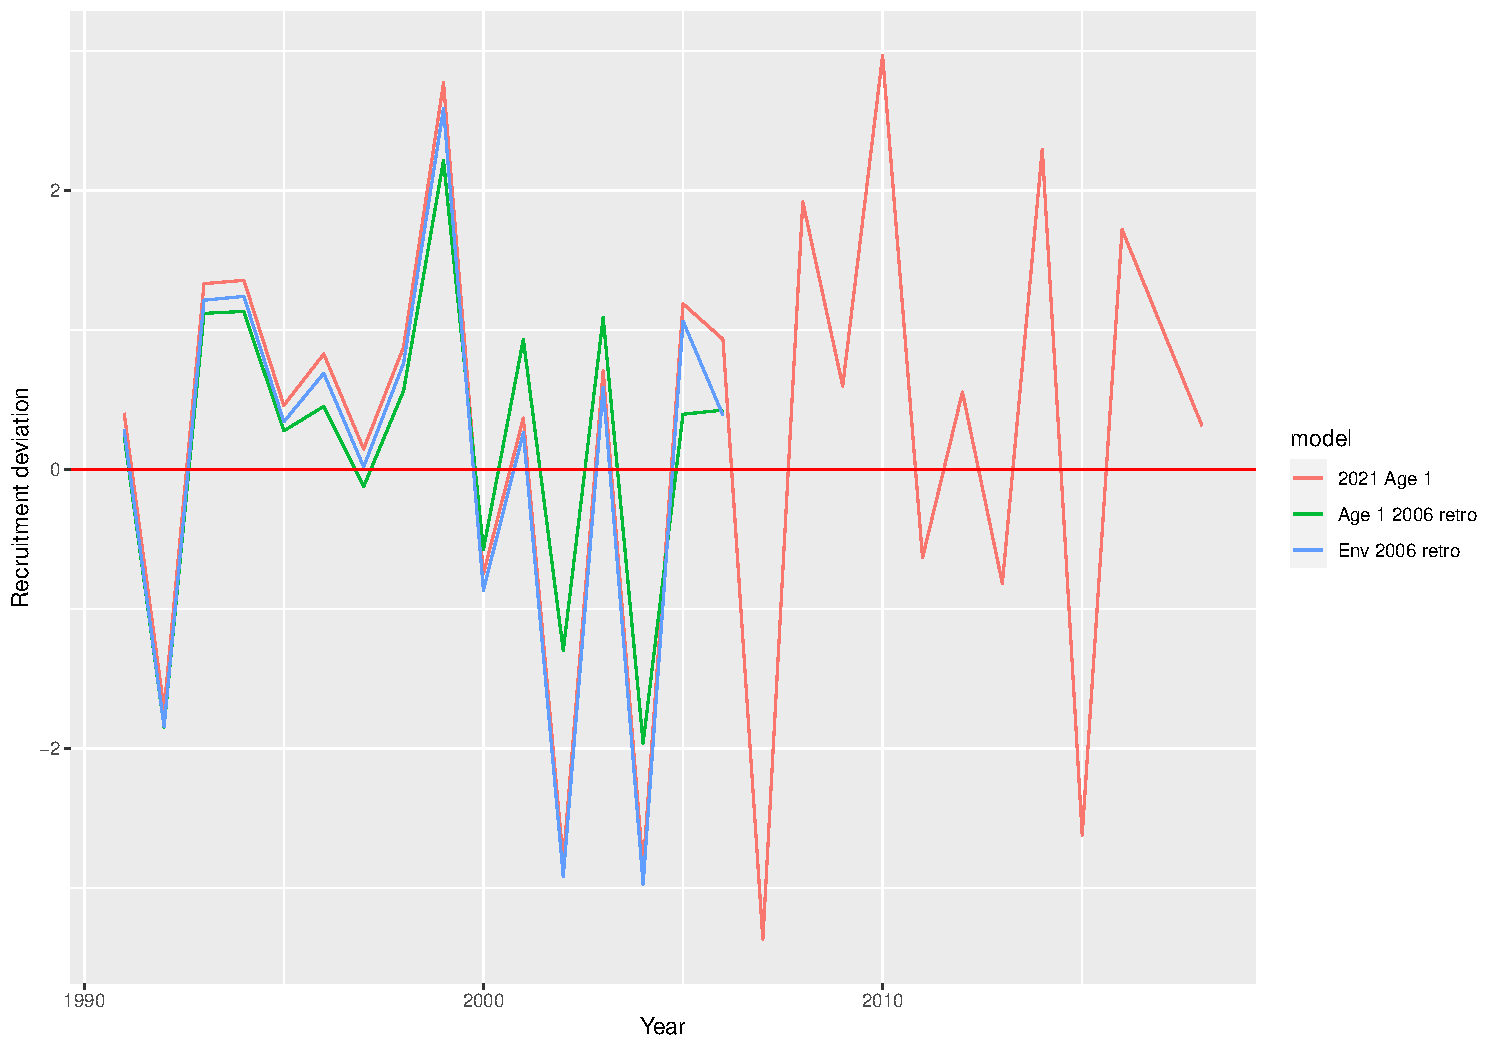
\includegraphics{presentation_files/figure-beamer/unnamed-chunk-3-1.pdf}

}

\end{figure}
\end{frame}

\begin{frame}
If there is no age-0 catch, what is informing the base retrospective
recruitment deviation in the terminal year?

\begin{figure}

{\centering \includegraphics[width=5.29167in,height=\textheight]{melpaper.PNG}

}

\end{figure}

\begin{figure}

{\centering \includegraphics[width=2.58333in,height=\textheight]{melpaperkey.PNG}

}

\end{figure}
\end{frame}

\begin{frame}
Three surveys used in the recruitment deviation likelihood estimation:
Fishery, Acoustic, Age-1

\begin{figure}

{\centering 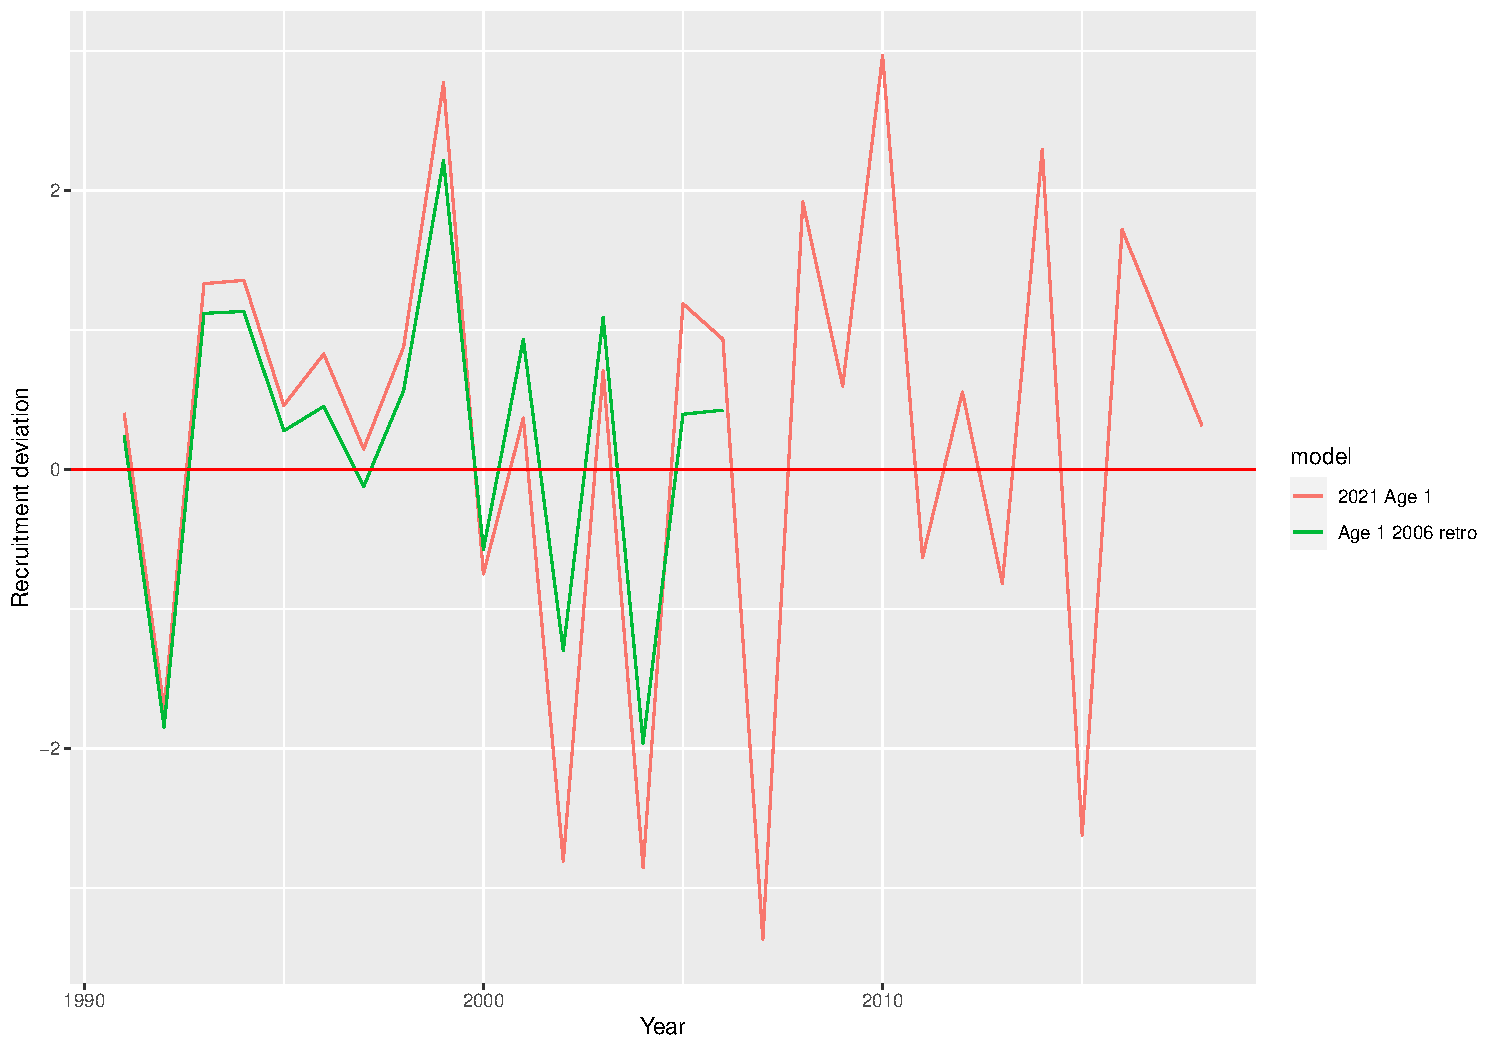
\includegraphics{presentation_files/figure-beamer/unnamed-chunk-4-1.pdf}

}

\end{figure}
\end{frame}

\begin{frame}
Only the age-1 survey is informing the recruitment deviation in the
terminal year

\begin{figure}

{\centering 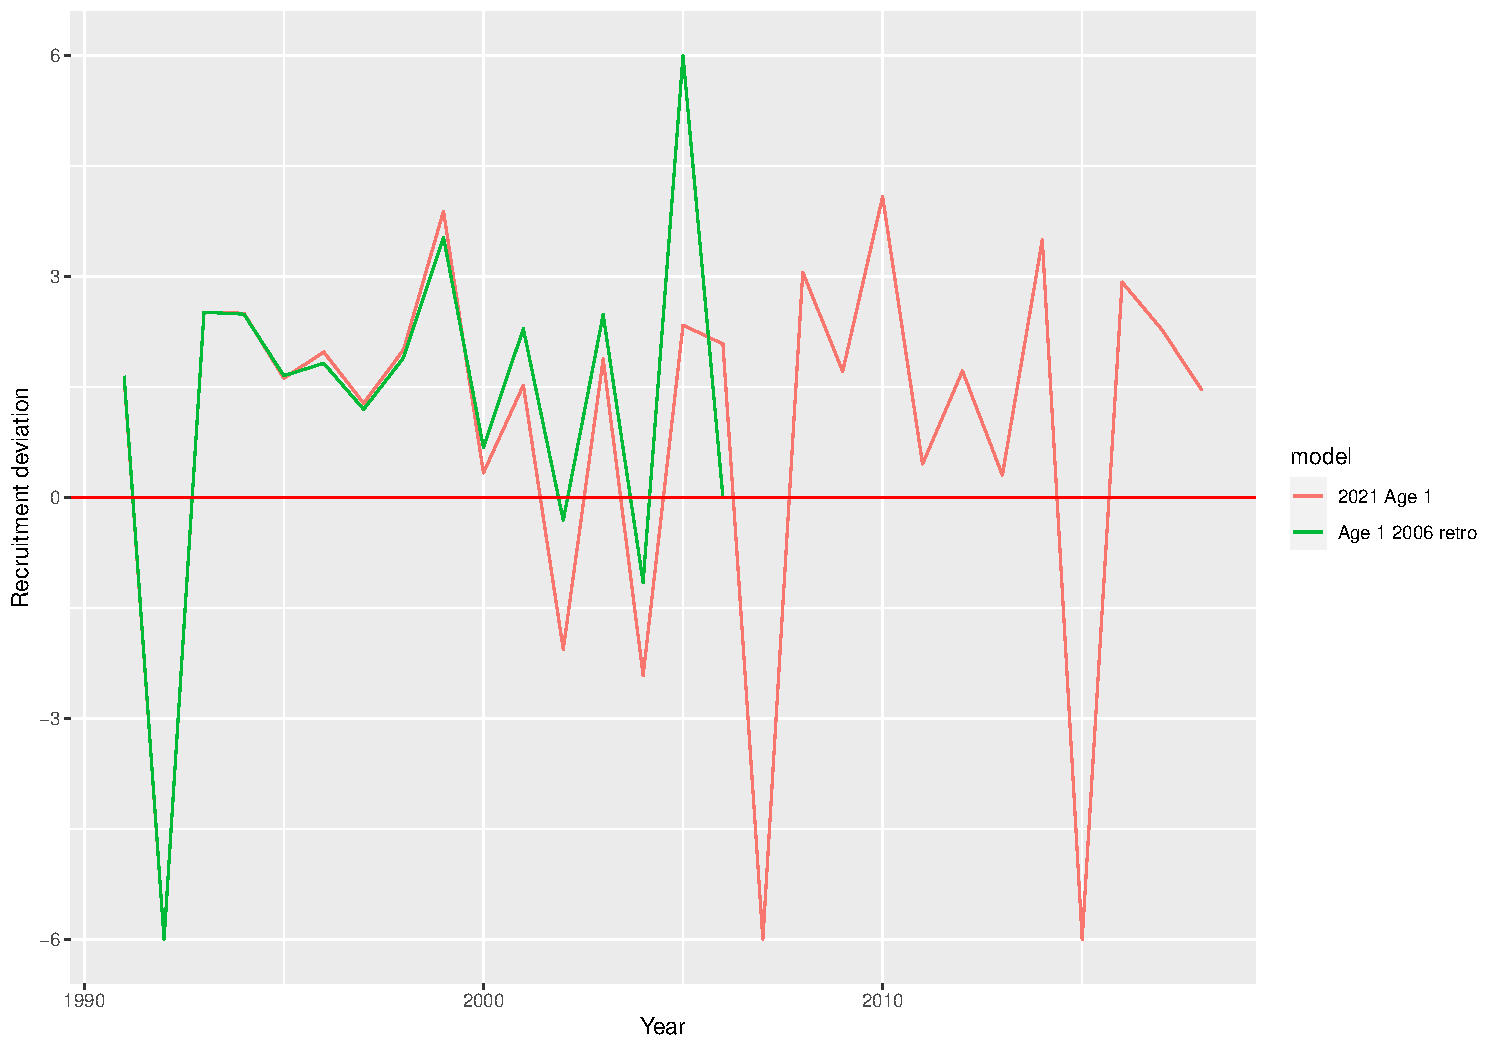
\includegraphics{presentation_files/figure-beamer/unnamed-chunk-5-1.pdf}

}

\end{figure}
\end{frame}

\begin{frame}[fragile]
Without the age-1 survey, inputting the rec devs for the environmental
driver performs very well:

\begin{figure}

{\centering 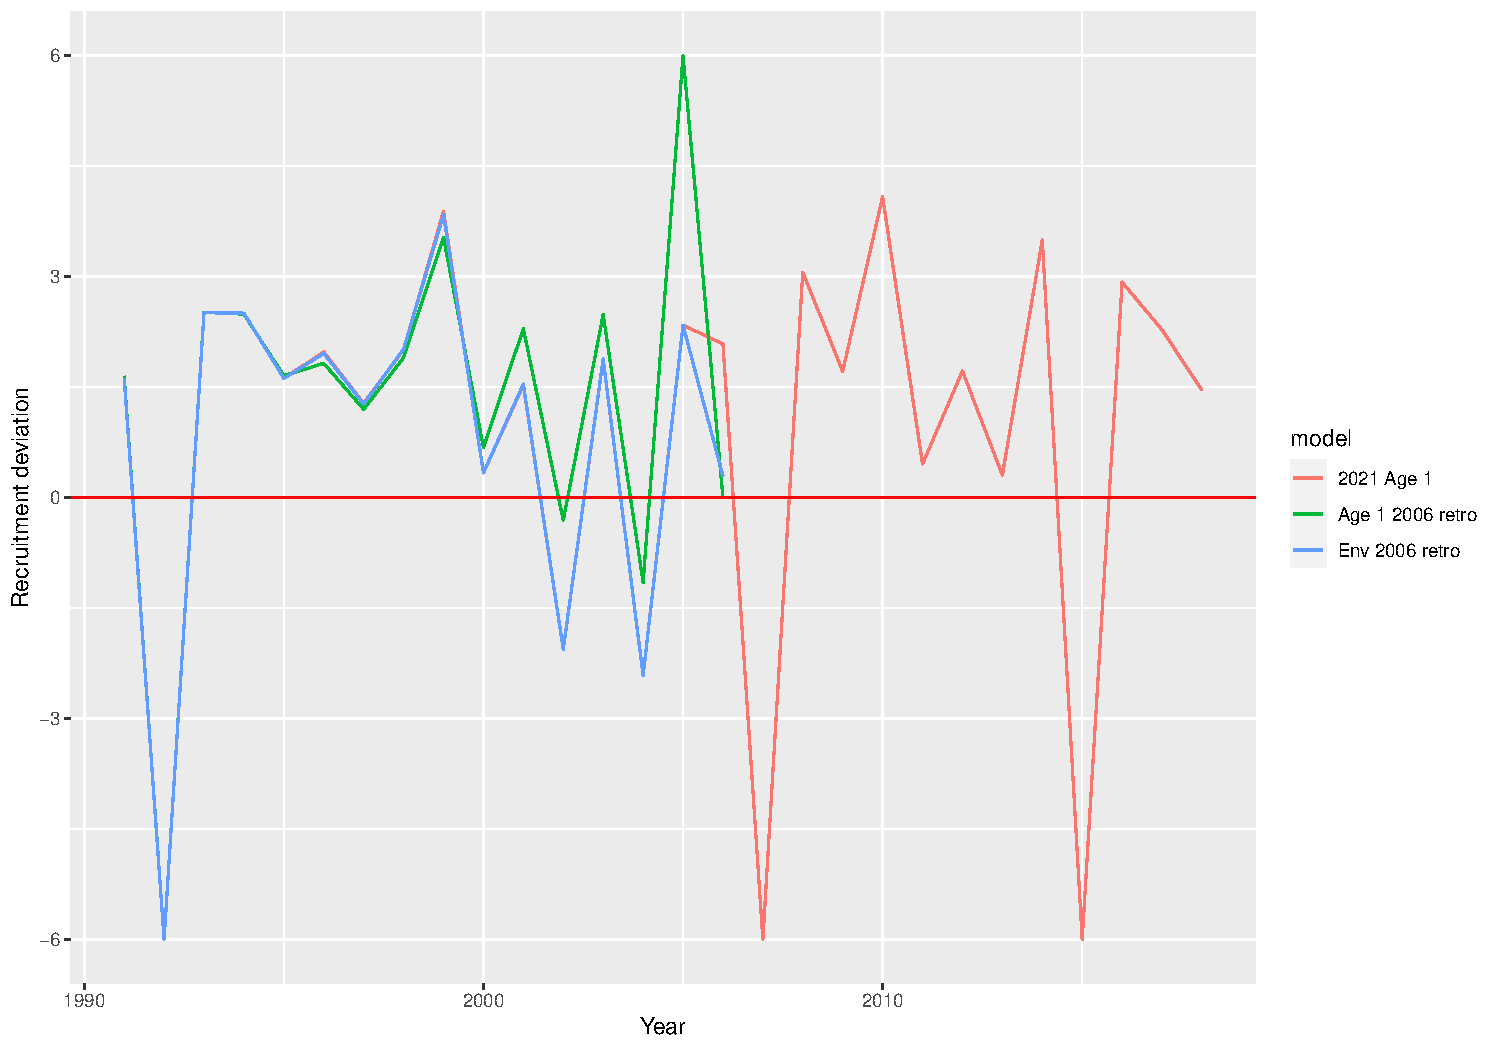
\includegraphics{presentation_files/figure-beamer/unnamed-chunk-6-1.pdf}

}

\end{figure}

\begin{block}{Discussion}
\protect\hypertarget{discussion}{}
What is happening in the terminal year for retrospective models?

\begin{Shaded}
\begin{Highlighting}[]
\NormalTok{r4ss}\SpecialCharTok{::}\FunctionTok{SS\_doRetro}\NormalTok{(}\AttributeTok{masterdir =} \FunctionTok{here}\NormalTok{(dirname),}
                 \AttributeTok{oldsubdir =} \StringTok{\textquotesingle{}\textquotesingle{}}\NormalTok{, }
                 \AttributeTok{years =} \SpecialCharTok{{-}}\NormalTok{peel,}
                 \AttributeTok{extras =} \StringTok{\textquotesingle{}{-}nohess\textquotesingle{}}
\NormalTok{)}
\end{Highlighting}
\end{Shaded}

Is there a better way to assess accuracy?
\end{block}

\begin{block}{Future explorations}
\protect\hypertarget{future-explorations}{}
\begin{itemize}
\tightlist
\item
  Using the model to estimate the added SE
\end{itemize}

\begin{figure}

{\centering 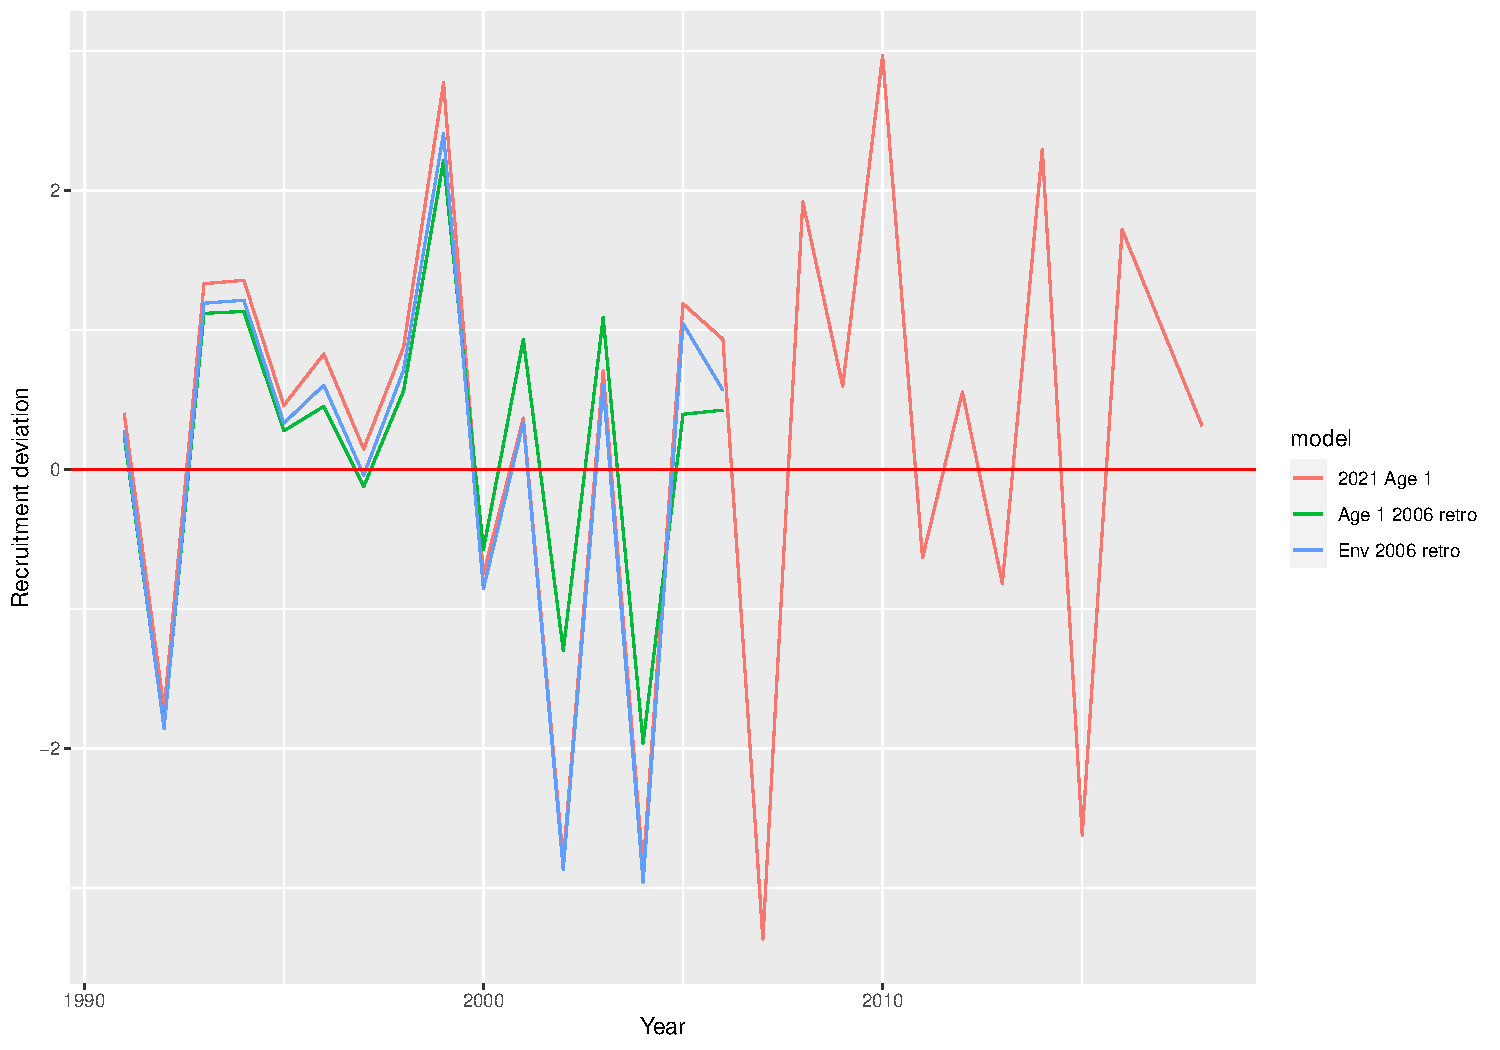
\includegraphics{presentation_files/figure-beamer/unnamed-chunk-8-1.pdf}

}

\end{figure}

\pause

\begin{itemize}
\tightlist
\item
  Simulate auto-correlated environmental drivers
\end{itemize}
\end{block}
\end{frame}

\begin{frame}{}
\protect\hypertarget{section}{}
\end{frame}



\end{document}
